\chapter{绪论}
本章首先介绍了软件定义网络的基础背景,随后介绍SDN当中的流量测量,以及现有的流量测量方式的局限,最后引出本文的研究内容。
\section{软件定义网络(SDN)}
随着互联网技术的高速发展,如今的互联网有着数据流量大、拓扑结构复杂、业务类型繁多的特点。
传统的网络结构体系在面对如今的互联网时逐渐显得力不从心,主要体现在维护困难、效率低、扩展性和兼容性不佳、安全性不足等。
传统网络中,每个路由器各自为战,通过一定的路由协议互相传递拓扑和链路信息,并独立维护一份信息。
这种方式的优点在于这样组成的网络是自组织的,在协议兼容的前提下可以轻易地向网络中加入结点,路由设施会自动完成路由表的更新。
而缺点在于,每个路由器所保存的拓扑信息和链路信息都是不完整的,很容易出现不同的源到同一目的的流量,由于路由算法汇聚到一起的现象,从而造成链路拥塞\cite{vissicchio2015central};
另一个问题是当设备或链路因为故障、维护、升级等原因出现变化,依靠路由协议传播变化信息耗时长且不稳定,可能会造成服务中断\cite{xu2018achieving}。

在这样的背景下,软件定义网络(Software-Defined Network, SDN)\cite{mckeown2008openflow}应运而生。
SDN的核心思想是将网络中的控制系统与数据转发系统分离开来,形成控制平面和数据平面两个平行的结构。
其中控制平面由一个或多个控制器组成,数据平面由众多交换机组成。控制器与交换机之间通过OpenFlow交流。
通过OpenFlow协议,SDN中的控制器可以得知整个网络的拓扑和统计信息,由此在全局层面维护整个网络。
SDN交换机与传统网络中的路由器存在较大的区别。第一,SDN交换机无需维护网络拓扑和链路信息。
SDN交换机中存放着一张或多张流表,每个数据包根据流表进行匹配并采取对应的操作。
当数据包无法匹配所有流表中的所有表项时,交换机会将该数据包上传给控制器,由控制器为其分配路径,并将路径转换为流表项下发至沿途的交换机中。
第二,SDN交换机可以对流进行精确匹配。传统路由器中的路由表是根据目的地址进行匹配的,而SDN中的流表项可以匹配各种各样的协议。
如TCP/UDP的源/目的端口、MPLS标记\cite{davie2000mpls}、ICMP报文类型、ARP操作类型(opCode)等都可以作为SDN流表项中的匹配域。
精密的匹配方式使得SDN可以实现对流的细粒度管理\cite{xu2017joint}。

通过使用OpenFlow与交换机通信,SDN的控制平面可以获取整个网络的几乎所有信息,管理交换机的各种行为。
这一特点使得SDN相比传统网络可以更加方便的部署各种应用,如服务链(Service Function Chain)\cite{halpern2015service}、QoS\cite{akella2014quality}等。

\begin{figure}[ht]
	\centering
	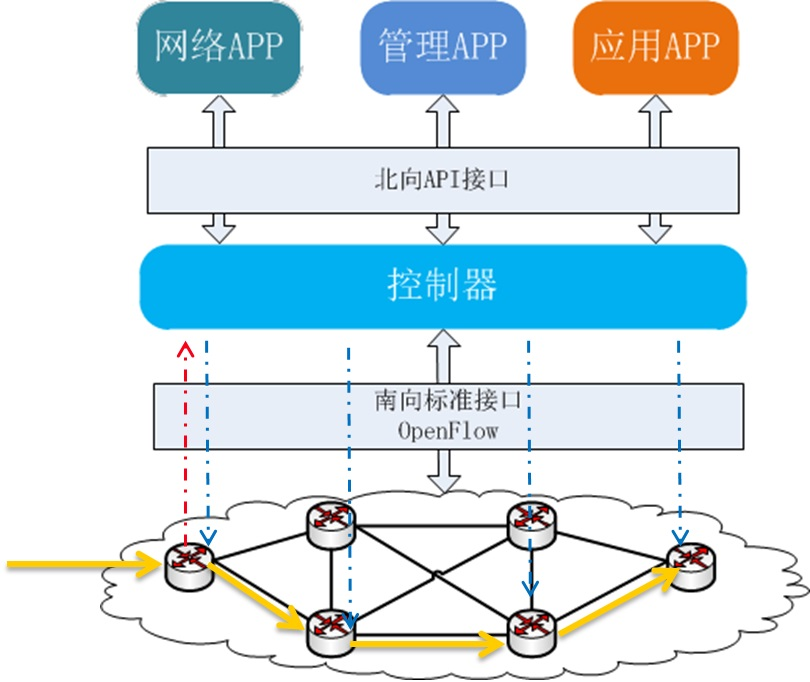
\includegraphics[width=0.8\linewidth]{fig/sdn.jpg}
	\caption{SDN网络结构}\label{fig:sdn}
\end{figure}

图\ref{fig:sdn}简要描绘了SDN的结构。图中的虚线表示了SDN中流表建立的过程。
最左侧的交换机收到一个无法匹配的数据包,通过红色虚线将其上传到控制器,控制器计算出路径后通过蓝色虚线将流表项下发给沿途的交换机,从而在网络中建立了一条新流。

\section{SDN中的流量测量}\label{sec:measurement}
为了实现网络的优化,流量统计信息对SDN是至关重要的。流的路由、QoS、入侵检测等应用都十分依赖于流的流量统计信息。
然而,SDN交换机的硬件资源限制了流量统计的能力,主要体现在以下三种重要的硬件资源上。
\textbf{第一种资源是三态内容寻址存储器(Ternary Content Addressable Memory, TCAM)。}
与普通的根据地址寻址的RAM不同,TCAM根据匹配字段的内容进行寻址,因而可以极快地完成查找和匹配的任务。
由于交换机要频繁地对流表进行匹配,因而往往使用TCAM来存储流表。
然而,TCAM的造价十分昂贵,并且非常耗电。受成本所限,交换机中配备的TCAM容量往往十分有限,这也导致交换机中的流表项条目数受限。
例如HP 5406zl型号交换机只能容纳1500条流表项\cite{curtis2011devoflow}。
\textbf{第二种资源是SRAM。}交换机中的SRAM扮演着主存储器的角色。受成本因素影响,中低端交换机的SRAM大小往往也很有限。
如Juniper入门款交换机仅仅有32MB的SRAM空间\cite{ResourceMonitoring},并且这仅有的SRAM上还承载着包括防火墙、路由控制在内的多种功能。
\textbf{第三种资源是CPU的计算资源。}SDN交换机最主要的功能是转发数据包,因此绝大多数的交换机都配备有专门的芯片用来转发数据包,以获得更高的吞吐率。
SDN交换机中的CPU则负责转发数据包之外的计算任务,因此其计算能力通常不高。市面上一些交换机的CPU仍在使用较为落后的MIPS指令集,主频甚至不足1GHz\cite{wang2014scotch}。

在SDN当中进行流量统计,目前主流有三种方法。第一种方法是使用交换机中的TCAM流表来进行统计。根据OpenFlow协议\cite{pfaff2012openflow},每个流表项当中都有一个字段用来统计符合该流表项的总流量。
然而如前所述,TCAM限制了流表项的条目数。即使是比较高端的Boradcom Trident2型号,其流表最多也只支持1.6万个条目\cite{cohen2014effect}。
而数据中心当中的流的数量动辄上百万\cite{kandula2009nature},1.6万个条目显然远远不够。
当网络中的流数超出流表上限时,常用的解决方法是将多条流通过规则整合的方式整合到一个流表项中\cite{zhao2018joint},如只匹配部分字段或使用掩码。
在这种情况下,流表项中统计的是符合该规则的所有流的流量,从而导致其中单个流的流量不得而知。

第二种方法是通过采样的方式进行统计,比如当前大多数交换机所支持的NetFlow\cite{estan2004building}或sFlow\cite{phaal2004sflow}解决方案。
然而,采样统计的测量精度常常不尽如人意\cite{yu2013software}\cite{li2016flowradar}。
提高采样统计的精度的最直接方法就是提高采样频率,但提高采样频率意味着消耗更多的计算和内存资源,从而影响此方案在有着更多流量的网络中的可伸缩性。

第三种方法是使用称为“Sketch”的数据结构进行流量统计。
在实际应用场景中,我们往往并不需要得知所有流的流量统计信息,而只关心其中一部分特殊流的信息。
通过特殊的算法,Sketch可以利用很少的内存空间来统计所有数据包,并且只留下关注的信息。
目前已经有很多种不同的Sketch被设计出来,分别适用于不同的使用场景,并在测量精确度和资源占用中取得平衡\cite{KXW06}\cite{li2012per}\cite{estan2002new}。

值得注意的是,目前为止的绝大多数流量测量方案都只关注数据平面的单个交换机,却很少考虑整个网络中的联合优化。
例如,现有的基于流表的统计方式中,每个交换机都会统计经过它的所有流。对于一条经过多个交换机的流而言,这种方案会带来非常大的冗余。
不过,由于交换机使用速度极快的TCAM存储流表,且所有数据包都必须匹配流表,流量统计只需要“顺便”累加一个计数器,因而这种冗余对性能的影响微乎其微。

然而当引入sketch之后,流量测量冗余的问题就凸显出来了。
因为sketch一般存放在SRAM中,且每处理一个数据包都要进行相对复杂的算法处理,所以sketch的计算负载不可能无限地降低,最终导致处理速度和流表相比始终会有较大差距。
此时,测量的冗余性所带来的计算负载变得不可小觑。
如果我们不再将视线聚焦于单个交换机,而是着眼于整个网络,那么则可以通过流量测量的分布式部署来对网络中的流量测量进行整体优化。

\section{文章结构}
根据第\ref{sec:measurement}节的介绍,本文的研究目标主要有以下三点:

第一点是设计一种能够测量大流流量的高效的Sketch。

对于SDN中的很多应用,往往最为关心的是如何获得网络中流量最大的若干条流的流量(也被称为top-$k$问题)。
例如,在实际场景中,控制器经常会向交换机部署默认路径以提升新流的响应速度,当许多流携带着大量流量同时经由默认路径转发时,网络中有可能会出现拥堵。
解决此问题的一种方案是,从这些通过默认路径的流当中找出其中流量较大的一些流,对它们进行重路由,从而实现更好的负载均衡。
因此,在交换机的层面,得知大流的较为准确的流量统计数据是非常重要的。
%其中设计的重点在于“高效”,也就是在不牺牲太多测量精度的前提下,尽量地减少Sketch本身的计算负载。
如前文所述,由于交换机的CPU性能较弱,且还需要负责执行OpenFlow控制协议以及其它维持交换机运行的必要功能,因此可分配给流量测量的计算资源极其有限。
如\cite{curtis2011devoflow}中的测量结果所示,即使在没有流量出入的情况下,测试用的交换机每秒只能完成275条流表项的设置。
假设包括Sketch在内的其它应用占用了50\%的CPU时间,那么每秒能处理的流表项数量只有137条,在面对较大流量时会不可避免出现性能瓶颈。

目前现有的一些通用Sketch,如UnivMon\cite{liu2016one},尽管可以获得所需的流量统计信息,但是受存储空间所限,不可能记录下所有的流的ID。
SketchVisor\cite{huang2017sketchvisor}、CountSketch\cite{charikar2004finding}和Filtered Space-Saving(FSS)\cite{homem2010finding}能够测量top-$k$的流并记录它们的ID,
但是在第\ref{chap:sketch}章中,根据我们的分析,这几种sketch的计算负载对于交换机而言仍然过大。
% 为了获得所需的流的ID,有的方案采取了对数据包头进行编码的方式,但这样又加重了交换机的计算负载。
% SketchVisor\cite{huang2017sketchvisor}设计了一个top-$k$的sketch,以及一个能够和其它sketch协作的框架,但是在流量较大的情况下它的计算负载仍然太大。
% 而如果单独使用它的top-$k$ sketch,在存储未命中的情况下则需要修改内存中的k个计数器,会带来无法接受的计算负载。

% CountSketch\cite{charikar2004finding}和Filtered Space-Saving(FSS)\cite{homem2010finding}是两种可以用来测量top-$k$流的sketch。
% 尽管它们可以分辨出大流的ID并记录这些大流的流量统计信息,但是这两种sketch的计算负载对于交换机而言仍然过大。
% 例如,CountSketch和FSS都需要在一个堆当中搜索某个给定的流ID是否存在。在不使用辅助数据结构的情况下,这个操作不得不遍历整个堆。具体的计算负载的分析将会在第\ref{chap:sketch}章中分析。

第二点是提出SDN中流量测量的分布式部署方案。分布式部署对于基于流表的测量并不必要,但是对于基于sketch的测量则是至关重要。
例如3条同样大小的流要经过同样的3台交换机,可以为每个交换机只分配1条流,这样每个交换机上的sketch只需要处理1/3的流量,进一步地减少了每个交换机上计算负载。
因而,我们需要对流量测量的分布式部署问题进行形式化建模和描述,并找出一个可以解决问题的算法。

最后一点则是sketch与分布式部署的结合实现。Sketch是运行在数据平面上的,而分布式部署的计算则依靠控制平面的整体信息。
只有二者协同工作,才能扬长避短,发挥sketch测量方法的优点。

在第\ref{chap:countmax}章,本文提出了名为“CountMax”的轻量级流量测量方案。与SketchVisor、CountSketch和FSS相比,CountMax具有以下优势:
\begin{enumerate}
    \item 测量精度高。在使用同样的内存空间时,CountMax的测量精度优于CountSketch和FSS约20\%。
    \item 存储占用低。CountMax不需要任何辅助数据结构,除了几十字节的元数据之外,占用的所有内存都是有效信息。
    \item 计算负载低。对每个到达的数据包,CountMax的每一“行”只需要执行一次哈希操作、一次比较操作和一次加法操作。
    \item 结构简单易于分布。一个CountMax sketch可以轻易地被拆分为多个,部署在不同的交换机上。通过安排每个交换机只处理一部分的流,可以将计算负载更平均地均摊到每个交换机之间。
\end{enumerate}
随后,本文在理论上证明了它的精确度和时间复杂度,并通过实验对CountMax的性能进行测试。

在第\ref{chap:gmsc}章中,我们提出了在每个交换机的计算资源有限的情况下最大化流统计覆盖的问题(MSC),并提出了解决此问题的算法GMSC。
随后通过实验结果证明了通过将分布式部署与sketch相结合,可以进一步降低单个交换机上的计算负载。



